% META %
\title{Trigonometry and a Sequence of Polynomials} % < This is the title of the paper.
\author{} % < This is the author of the paper.
\date{August 2018} % < Alternately use this as subtitle or course number!

% PACKAGES AND SETTINGS %
\documentclass[12pt, letterpaper]{article} % for a4 sized paper, define a4paper instead of letterpaper
\usepackage[utf8]{inputenc}
\usepackage[english]{babel}
\usepackage[bottom]{footmisc}
\usepackage{amsmath}
\usepackage{amsfonts}
\usepackage{mathpazo} % text font is mathpazo
\usepackage[notext, lighttext, intlimits]{kpfonts} % math font is kp-fonts
\usepackage[T1]{fontenc}
\usepackage{microtype} % optimizes spacing for text
\usepackage{pgfplots}
\usepackage{geometry}
\usepackage{amsthm}
\newtheorem{theorem}{Property}
\newtheorem{conjecture}{Conjecture}
\geometry{ % defines page margins and spacing
  top=0.95in,
  inner=1.2in,
  outer=1.2in,
  bottom=1.2in,
  headsep=2ex,
  foot=36pt}
\makeatletter
\usepackage{lastpage,fancyhdr,graphicx}
\usepackage{epstopdf}
\pagestyle{myheadings}
\pagestyle{fancy}
\fancyhf{}
\lhead{\@title}
\rhead{\@author}
\lfoot{\small{\today}}
\rfoot{\small{\textsc{p. \thepage/\pageref{LastPage}}}}
\renewcommand{\footrule}{\hrule height 1.3pt \vspace{1.3mm}}
\headsep = 0.25in
\fancyheadoffset[R]{0.35in}
\fancyheadoffset[L]{0.35in}
\fancyfootoffset[R]{0.35in}
\fancyfootoffset[L]{0.35in}
\begin{document}

% DOCUMENT TITLE SECTION %
\begin{center}
	\ \\
	\vspace{120pt}
	\textsf{\huge\@title}\\[12pt]
Jiahua Chen, Sivabalan Muthupalaniappan, Andrew Wu, Medha Yelimeli
\\ Counselor - Arya Vadnere
\\[6pt]
	\@date
	\makeatother
	\\
\end{center}

% BODY %
\vspace{20pt}
\begin{abstract}
We explore a sequence of polynomials related to the expansion of $\cos (nx)$ for natural numbers $n$. We analyze various patterns concerning the coefficients of these polynomials, along with a recursive formula to build later polynomials from earlier polynomials. In addition, we conjecture explicit formulas for these polynomials as well as polynomials related to the expansions of $\sin (nx)$ and $\tan (nx)$ and prove a different explicit formula using generating functions. Finally, we perform visual analyses of the graphs of the polynomials and their behaviour when taken modulo $p$ for odd primes $p$. \\
\end{abstract}
\vspace{20pt}
\textbf{Acknowledgments} \\

We thank \textbf{Arya Vadnere} for his guidance and expertise. \\

We also thank the \textbf{PROMYS} program for this wonderful opportunity to explore this topic in-depth.



\newpage
\tableofcontents{}
\newpage
\section{Introduction}
Consider the expression $\cos (nx)$ for non-negative integers $n$. When $n \ge 2$, we can break this expression down using the cosine addition formula; namely, $\cos (a+b) = \cos(a)\cos(b) - \sin(a)\sin(b)$. For example,
\begin{align*}
\cos (2x) & = \cos (x + x) \\
 & = \cos(x) \cos(x) - \sin(x)\sin(x) \\
 & = \cos^2(x) - \sin^2(x) \\
 & = \cos^2(x) - (1 - \cos^2(x)) \\
 & = 2\cos^2(x) - 1. \\
\intertext{
Here we used the fact that $\sin^2(x) + \cos^2(x) = 1$. Observe that the final expression is a polynomial in $\cos(x)$. We show one more example:
}
\cos(3x) & = \cos(2x + x) \\
    & = \cos(2x) \cos(x) - \sin(2x)\sin(x) \\
    & = (2 \cos^2(x) - 1)\cos(x) - 2\sin(x)^2\cos(x) \\
    & = 2\cos^3(x) - \cos(x) - 2(1 - \cos^2(x))\cos(x) \\
    & = 4\cos^3(x) - 3\cos(x). \\
\end{align*}
Once again, the result is a polynomial in $\cos(x)$. Considering this, we might try to define a function $T_n(u) = \cos(nx)$ such that $u = \cos(x)$. This definition yields that as $\cos(2x) = 2\cos^2(x) - 1$, $T_2(u) = 2u^2 - 1$. Similarly $T_3(u) = 4u^3 - 3u$. \\

We now show the first few values of $T_n(x)$, computed by the same methods as shown above.

 \begin{align*}
  T_0(u) & = 1                                      \\
  T_1(u) & = u                                      \\
  T_2(u) & = 2u^2 - 1                               \\
  T_3(u) & = 4u^3 - 3u                              \\
  T_4(u) & = 8u^4 - 8 u^2 + 1                       \\
  T_5(u) & = 16u^5 - 20u^3 + 5u                     \\
  T_6(u) & = 32u^6 - 48u^4 + 18u^2 - 1              \\
  T_7(u) & = 64u^7 - 112u^5 + 56u^3 - 7u            \\
  T_8(u) & = 128u^8 - 256u^6 + 160u^4 - 32u^2 + 1   \\
  T_9(u) & = 256u^9 - 576u^7 + 432u^5 - 120u^3 + 9u
 \end{align*}

Given these initial examples, we can already find a handful of patterns: it appears that $T_n(u)$ is always a polynomial of degree $n$, and that its leading term has coefficient $2^{n-1}$. Furthermore, the coefficients are all of even degree if the polynomial is of even degree, and all of odd degree if the polynomial is of odd degree. \\

It turns out that there are many more non-trivial properties regarding that coefficients of these polynomials, all of which can be proven by the following recursive formula:

\begin{theorem} \[T_n(u) = 2u\cdot T_{n-1}(u) - T_{n-2}(u)\] \end{theorem}

\begin{proof}
We use the identity $\cos a + \cos b = 2\cos(\frac{a+b}{2})\cos(\frac{a-b}{2})$.

Let $a = nx$, $b = (n-2)X$. Substituting, we get:

\[\cos(nx) + \cos((n-2)x) = 2 \cos((n-1)x) \cos x\]

Substituting for $T_n$ and $u = \cos x$, we have $T_{n}(u) + T_{n-2}(u) = 2u\cdot T_{n-1}(u)$, which is precisely what we wanted to prove.
 \end{proof}

Observe that this formula is proven only using trigonometry, essentially. There are a few more properties we can show without referencing the recursive formula, which we will prove below.

\begin{theorem} $T_{2n}(u) = 2T_{n}(u)^2 - 1.$ \end{theorem}

\begin{proof} We have $\cos{(2nx)} = \cos(nx + nx)$, which reduces to $2\cos^2(nx) - 1$ after applying the double angle formula. \end{proof}

\begin{theorem} $T_{pq}(u) = T_p(T_q(u)) = T_q(T_p(u)).$ \end{theorem}

\begin{proof} We can write $\cos(pqx) = T_{pq}(\cos x)$, or as $T_p(\cos(qx))$, or as $T_q(\cos(px))$. \end{proof}


\begin{theorem}
$T_n(1) = 1$.
\end{theorem}

\begin{proof}
Observe that $\cos (n \cdot 0) = 1$ for all $n$, and that $\cos (nx) = T_n(u)$. We are done.
\end{proof}

\begin{theorem}
The roots of $T_n(u)$ are $u = \cos \left(\frac{(2k-1)\pi}{2n}\right)$ for $1 \le k \le n$.
\end{theorem}

\begin{proof}
We know that $\cos (nx) = T_n(u)$. But $\cos (nx) = 0$ when $nx$ is an odd multiple of $\pi / 2$, or when $x = \frac{(2k-1)\pi}{2n}$. But $u = \cos x$, done.
\end{proof}

\newpage
\section{Justifying our Initial Observations}

Now we will prove a number of interesting properties about the coefficients of the terms in $T_n(u)$, using the recursive formula we found earlier. \\

\begin{theorem}
$T_n(u)$ is a integer polynomial of degree $n$; all its terms are of odd or even degree; the coefficient of the $u^n$ term is $2^{n-1}$ for $n \ge 1$; the coefficient of the $u^{n-2}$ term is $-2^{n-3}\cdot n$ for $n \ge 3$.
\end{theorem}

\begin{proof} We provide an inductive proof for all these properties.

We observe firstly, as a base case, that $T_0(u)$ and $T_1(u)$ are polynomials in $\mathbb{Z}[u]$. Next, suppose that $T_{k}(u)$ and $T_{k+1}(u)$ are polynomials in $\mathbb{Z}[u]$. Then $T_{k+2}(u) = 2u \cdot T_{k+1}(u) - T_{k+2}(u)$, and as $\mathbb{Z}[u]$ is closed under addition and multiplication, $T_{k+2}(u) \in \mathbb{Z}[u]$. Furthermore, $T_0(u)$ and $T_1(u)$ are polynomials of degree $0$ and $1$, respectively; next, if $T_k(u)$ and $T_{k+1}(u)$ are of degree $k$ and $k+1$, respectively, then $T_{k+2}(u)$ must be of degree $k+2$ because we multiply $T_{k+1}(u)$ by $2u$. \\

Next, we see that the coefficient of the $u^1$ term in $T_1(u)$ is indeed $2^0 = 1$. Now we proceed to the inductive step: suppose that the coefficient of $u^k$ in $T_k(u)$ is $2^{k-1}$. Then $T_{k+1}(u) = 2u \cdot T_k(u) - T_{k-1}(u)$, so the coefficient of $u^{k+1}$ is $2^k$ (subtracting $T_{k-1}(u)$ does not impact the leading coefficient because it has degree $k-1$.)\\

Finally, we induct on the last sub-property. For $n = 3$, $T_3(u) = 4u^3 - 3u$, so the coefficient of the $u$ term is indeed $-2^0 \cdot 3 = -3$. Next, we proceed to the inductive step: suppose that the coefficient of the $u^{n-2}$ term is $-2^{n-3}\cdot n$ for $n = k$. We will show that the coefficient of the $u^{k-1}$ term is $-2^{k-2}\cdot (k+1)$ in $T_{k+1}(u)$.\\

We know already that $T_{k+1}(u) = 2u \cdot T_k(u) - T_{k-1}(u)$. By previous work, we know that the coefficient of the $u^{k-1}$ term in $T_{k-1}(u)$ is $2^{k-2}$; furthermore, the coefficient of the $u^{k-2}$ term in $T_{k}(u)$ is $-2^{k-3} \cdot k$ by the inductive hypothesis. If we multiply this by $2$, we get $-2^{k-2} \cdot k$. Subtracting another $2^{k-2}$ from this yields $-2^{k-2} \cdot (k+1)$, as desired, so our induction is complete.
\end{proof}

\begin{theorem}
The coefficient of the $u^0$ term in $T_{2k}(u)$ is $1$ if $k$ is even and $-1$ if $k$ is odd.
\end{theorem}

\begin{proof}
Observe that substituting in $u = 0$ is equivalent to substituting $\cos (x) = 0$, or equivalently, $x = \frac{(2k+1)\pi}{2}$ with $k \in \mathbb{Z}$. But then $\cos (nx) = \cos \frac{n(2k+1)(\pi)}{2}$, so if $n\equiv 0 \pmod{4}$, we get an even multiple of $\pi$, giving us $1$. If $n \equiv 2 \pmod{4}$, we get an odd multiple of $\pi$, giving us $-1$. We finish by observing that if $k$ even and $n \equiv 0 \pmod{4}$ are equivalent because $n = 2k$, and similarly $k$ odd and $n \equiv 2 \pmod{4}$ are equivalent.
\end{proof}

\newpage
\begin{theorem}
The coefficient of the $u^1$ term in $T_{2k+1}(u)$ is $2k+1$ if $k$ is even and $-(2k+1)$ if $k$ is odd.
\end{theorem}

\begin{proof}
We induct. The base cases are shown in the example polynomials we provided.

Now assume that this property holds for $k = 0,1,2,\cdots ,n$ where $n$ is odd. We show it holds for both $k = n+1$ and $n+2$. \\

We want to show that the coefficient of the $u$ term in $T_{2n+3}(u)$ is $2n+3$, firstly. But $T_{2n+3}(u) = 2uT_{2n+2}(u) - T_{2n+1}(u)$. As the coefficient of the $u$ term in $T_{2n+1}(u)$ is $-(2n+1)$ by the inductive hypothesis, and as the coefficient of the $u^0$ term in $T_{2n+2}(u)$ term is $1$ by the previous property and the fact that $n$ is odd, we know that the $u$ term's coefficient in $T_{2n+3}(u)$ is $2 - (-(2n+1)) = 2n + 3$ as desired.\\

Now we show that the coefficient of the $u$ term in $T_{2n+5}(u)$ is $-(2n+5)$. By our recursive formula, $T_{2n+5}(u) = 2uT_{2n+4}(u) - T_{2n+3}(u)$. The coefficient of $u$ in $T_{2n+3}(u)$ is $2n+3$, by previous work, and the coefficient of the $1$ term in $T_{2n+4}(u)$ is $-1$ by the previous property. Then we get that the $u$ term has coefficient $2(-1) - (2n+3) = -2n - 5$ as desired.
\end{proof}

\begin{theorem} The coefficient of the $u^2$ term in $T_{2k}(u)$ is $-2k^2$ if $k$ is even and $2k^2$ if $k$ is odd.
\end{theorem}

\begin{proof}
We proceed by induction. The base cases were shown above as examples.

Next, assume the property holds for $k = 0,1,2,\cdots ,n$. We show it holds for $k = n+1$ and $k = n+2$. Assume $n$ is odd. \\

We want to show that the coefficient of the $u^2$ term in $T_{2(n+1)}(u)$ is $-2(n+1)^2$. We have $T_{2(n+1)}(u) = 2uT_{2n+1}(u) - T_{2n}(u)$. The coefficient of the $u$ term in $T_{2n+1}(u)$ is $-(2n+1)$ by the previous property; the coefficient of the $u^2$ term in $T_{2n}(u)$ is $2n^2$. Then $2(-(2n+1)) - 2n^2 = -2(2n+1+n^2) = -2(n+1)^2$, as desired.\\

Next, we want to show that the coefficient of the $u^2$ term in $T_{2(n+2)}(u)$ is $2(n+2)^2$. We know that $T_{2(n+2)}(u) = 2uT_{2n + 3}(u) - T_{2n + 2}(u)$. As the coefficient of the $u$ term in $T_{2n+3}(u) = T_{2(n+1)+1}(u)$ is $2(n+1) + 1$ by the previous property, and as the coefficient of the $u^2$ term in $T_{2n+2}(u)$ is $-2(n+1)^2$, so the coefficient of the $u^2$ term in $T_{2(n+2)}(u)$ is $2(2(n+1) + 1) - (-2(n+1)^2) = 4n + 6 + 2n^2 + 4n + 2 = 2(n+2)^2$, as desired.
\end{proof}

\begin{theorem}
The coefficient of the $u^3$ term in $T_{2k-1}(u)$ is $\binom{2k}{3}$ if $k$ is even and $-\binom{2k}{3}$ if $k$ is odd.
\end{theorem}

\begin{proof}
By the same induction methods as before, it suffices to show that $\binom{2k+2}{3} = 2(2k^2) + \binom{2k}{3}$. It suffices to show this for both $k$ even and $k$ odd because negatives cancel.\\

Using the formula for $\binom{a}{b}$ yields that we must show that
$$\dfrac{(2k+2)(2k+1)(2k)}{6} = 4k^2 + \dfrac{(2k)(2k-1)(2k-2)}{6},$$
which is true upon expansion.
\end{proof}

\section{Observing $\sin(nx)$ and $\tan(nx)$}
Having proven many properties of the polynomials $T_n(u)$ using the recursive formula, we now generalize: we look into polynomials involving $\sin (nx)$ and $\tan (nx)$, and we conjecture and prove a few explicit formulas. \\

\begin{theorem}
For all $n \in \mathbb{N}$, $\sin{(nx)}$ can be expressed as $\sin x \cdot P(\cos x)$, where $P$ is a polynomial with integer coefficients.
\end{theorem}

\begin{proof}
We proceed by induction. The base case is $\sin x = \sin x \cdot 1$, which satisfies the property for $P = 1$. Now assume that $\sin ((n-1)x) = \sin x \cdot P(\cos x)$ for some polynomial P with integer coefficients. By the angle sum identity,
$$ \sin(nx) = \sin((n-1)x + x) = \sin((n-1)x)\cos(x) + \cos((n-1)x) \sin x$$
We know $\cos((n-1)x) = T_{n-1}(\cos x)$, which we have proven is a polynomial in $\cos(x)$ with integer coefficients. Moreover, by our inductive hypothesis, we can write $\sin((n-1)x) = \sin(x) \cdot P(\cos(x))$. Substituting, we have:

$$ \sin(nx) = \sin(x) \cdot P(\cos(x)) \cdot \cos(x) + T_{n-1}(\cos x) \cdot \sin(x)$$
$$ = \sin(x) \cdot \big( P(\cos(x)) \cdot \cos x + T_{n-1}(\cos x) \big)$$

And since $P(\cos x)$, $\cos x$, and $T_{n-1}(\cos x)$ are polynomials in $\cos x$, the induction is complete.
\end{proof}

Motivated by this result, we look into the quotient $S_n(u) = \frac{\sin (nx)}{\sin x}$, which we now know is a polynomial. Plugging in $n = 1$ yields $S_1 = 1$. Again, we will demonstrate the calculation for $n = 2$ and $n=3$. Observe that
\begin{align*}
\sin (2x) & = \sin (x + x) \\
 & = \sin (x) \cos(x) + \sin (x)\cos(x) \\
 & = 2\sin x \cos x. \\
\intertext{
Thus $\frac{\sin(2x)}{\sin{x}} = 2\cos x \implies S_2(u) = 2u$. Now we compute $\frac{\sin(3x)}{\sin x}$:
}
\sin(3x) & = \sin(2x + x) \\
    & = \sin(2x) \cos(x) + \sin(x)\cos(2x) \\
    & = 2\sin(x) \cos^2(x) - \sin(x)(2\cos^2(x) - 1) \\
    & = 2\sin(x) (4\cos^2(x) - 1) \\
\end{align*}
which yields $\frac{\sin(3x)}{\sin(x)} = 4\cos^2(x) - 1$, from which it follows that $S_3(u) = 4u^2 - 1$. \\

We investigate possible recurrences, as in our polynomials for $\cos (nx)$, and find that $S_n(u)$ satisfies the same recurrence as $T_n(u)$.

\begin{theorem}
Let $S_{n}(u)=\frac{\sin(nx)}{\sin{x}},\text{ where } u = \cos x$. The first few $S_{n}$ are as follows.

\begin{align*}
S_{1} &= 1 \\
S_{2} &= 2u \\
S_{3} &= 4u^{2} -1 \\
S_{4} &= 8u^{3} - 4u \\
S_{5} &= 16u^{4} - 12u^{2} + 1 \\
S_{6} &= 32u^{5} - 32u^{3} + 6u
\end{align*}

Specifically, we have that $S_{n} = 2u\cdot S_{n-1} - S_{n-2}$.
\end{theorem}

\begin{proof}
It suffices to show that $\dfrac{\sin ((n+2)x)}{\sin(x)} = 2\cos (x) \cdot \dfrac{\sin ((n+1)x)}{\sin (x)} - \dfrac{\sin (nx)}{\sin (x)}$ for $n \ge 0$. Multiply through by $\sin (x)$, such that we want to show
$$\sin ((n+2)x) = 2\cos (x) \cdot \sin ((n+1)x) - \sin (nx).$$
We know that
\begin{align*}
\sin((n+2)x) & = \sin((n+1)x + x) \\
& = \sin((n+1)x)\cos(x) + \sin(x)\cos((n+1)x) \\
\end{align*}
by the addition formula. After substituting this and subtracting $\sin((n+1)x)\cos(x)$ from both sides, it suffices to show that
$$\sin(x) \cos((n+1)x) = \cos(x) \sin ((n+1)x) - \sin(nx).$$
We also know that
$$\sin(x)\cos((n+1)x) - \cos(x)\sin((n+1)x) = \sin(-nx)$$
by the subtraction formula. But $\sin(-nx) = -\sin(nx)$, done.
\end{proof}

\section{Explicit Formulas}
We also looked into finding explicit formulas for $T_n(u)$ and $S_n(u)$. \\

\begin{conjecture}An explicit form for the original Chebyshev polynomials is given by $$T_n(u) = \displaystyle\sum_{k=0}^{\left\lfloor \tfrac{n}{2} \right\rfloor} \left[(u^2-1)^k \cdot u^{n-2k} \cdot \binom{n}{2k}\right].$$\end{conjecture}

\begin{conjecture}
An explicit form for $S_{n}$ is given by
$$ S_{n}(u) = \displaystyle\sum_{k=0}^{\left\lfloor \tfrac{n-1}{2} \right\rfloor} \left[(-1)^k \cdot (2u)^{n-1-2k} \cdot \binom{n-k-1}{k}\right]$$
where $u = \cos{x}$.
\end{conjecture}

\begin{conjecture}
We also have
$$A_n(v) = \dfrac{\displaystyle\sum_{j=0}^{\left\lfloor \frac{n-1}{2} \right\rfloor} (-1)^j \cdot \binom{n}{2j + 1}\cdot v^{2j + 1}}{\displaystyle\sum_{j=0}^{\left\lfloor \frac{n}{2} \right\rfloor} (-1)^j \cdot \binom{n}{2j}\cdot v^{2j}}$$
where $A_n(v) =  \tan(nx)$ and $v=\tan(x)$.
\end{conjecture}

\begin{conjecture} Let $n \in \mathbb{N}$ be odd. Then
$$ \sin(nx) = (-1)^{\frac{n-1}{2}}\cdot  T_{n}(\sin x)$$
where $T_{n}$ is defined as above. \end{conjecture}

\begin{conjecture}
Let $n \in \mathbb{N}$ be even. Then
$$ \sin(nx) = (-1)^{\frac{n}{2}-1} \cdot \cos x \cdot S_{n}(\sin x)$$
where $S_{n}$ is defined as above.
\end{conjecture}
\newpage
\section{Generating Functions}
We now look into a different explicit formula for $T_n$, this one found using generating functions.\\

\begin{theorem}
$$ T_{n}(u) = \frac{1}{2} \left[ \frac{1}{(u+\sqrt{u^{2}-1})^{n}} + \frac{1}{(u-\sqrt{u^{2}-1})^{n}} \right]$$
\end{theorem}

\begin{proof}
We begin by defining a generating function for $T_{n}(u)$: Let $f(x) = \displaystyle \sum_{n=0}^{\infty} T_{n}x^{n}$. That is, $f(x) = 1 + ux + (2u^2-1)x^2 + (4u^3-3u)x^3 + \cdots + T_{n}x^{n}+\cdots$. (We use the shorthand $T_k = T_k(u)$ here.)
Motivated by our recurrence, we now consider $2uxf(x) = 2ux + (2u^2)x^2 + (4u^2-2u)x^3 + \cdots + 2uT_{n}x^{n+1}$. Subtracting $f(x)$ yields
$$(2ux-1)f(x) = -1 + ux + x^{2} + ux^{3} +(2u^{2}-1)x^{4} + (4u^{3}-3u)x^{5} + \cdots + T_{n}x^{n+2}+\cdots$$
But the right-hand-side is precisely $(-1 + ux) + x^{2}f(x)$. Solving for $f(x)$, we have $f(x) = \frac{1-ux}{1-2ux+x^2}$.
At this point, we use the method of partial fractions: suppose that $1 - 2ux + x^2$ has roots $p$ and $q$, such that its factorization is $(x-p)(x-q) = 1 - 2ux + x^2$. Then we need to solve the equation
$$\dfrac{A}{x-p} + \dfrac{B}{x-q} = \dfrac{1 - ux}{1 - 2ux + x^2}.$$
Define two new variables $A'$ and $B'$ such that $A' = -Ap$ and $B' = -Bq$. Then it's equivalent to solving
$$A'\cdot \left( \dfrac{1}{1 - \frac{x}{p}} \right)+ B' \cdot \left( \dfrac{1}{1- \frac{x}{q}} \right) = \dfrac{1 - ux}{1 - 2ux + x^2} = f(x).$$
Note that we can rewrite some terms as geometric series, such that
$$A' \cdot \displaystyle\sum_{k=0}^{\infty} \left(\frac{x}{p}\right)^k + B' \cdot \displaystyle\sum_{k=0}^{\infty} \left(\frac{x}{q}\right)^k = f(x).$$
At this point, we may equate coefficients: for all $k$, we have $A' \cdot \left( \frac{1}{p} \right)^k + B' \cdot \left( \frac{1}{q} \right)^k = T_k$. Substituting $k = 0$ and $k = 1$ yields the equations
$$A' + B' = 1$$
$$\frac{A'}{p} + \frac{B'}{q} = u.$$
Note now that we can actually solve for $p$ and $q$ in terms of $u$, by using the quadratic formula. We also make the substitution $B' = 1 - A'$, yielding
$$\frac{A'}{u + \sqrt{u^2 + 1}} + \frac{1 - A'}{u - \sqrt{u^2 - 1}} = u.$$
Continuing, we have
$$A'(u - \sqrt{u^2 - 1}) + (1-A')(u + \sqrt{u^2 - 1}) = u(u^2 - *u^2 - 1)).$$
Upon simplification, this reduces to
$$A' \sqrt{u^2 - 1} + A' \sqrt{u^2 - 1} = \sqrt{u^2 - 1}$$
which in turn yields that $A' = B' = \frac{1}{2}$.
Hence $A' \cdot \left( \frac{1}{p} \right)^k + B' \cdot \left( \frac{1}{q} \right)^k = T_k$ implies, after substitution and a change of variables, that a general formula for $T_n(u)$ is
$$T_{n}(u) = \frac{1}{2} \left[ \frac{1}{(u+\sqrt{u^{2}-1})^{n}} + \frac{1}{(u-\sqrt{u^{2}-1})^{n}} \right]$$
as desired.
\end{proof}

\section{Coefficients Modulo Prime \emph{p}}
We also want to investigate the original polynomials for $\cos(nx)$ modulo primes $p$. We conjectured the following result:

\begin{conjecture} If we work in $\mathbb{Z}_p[u]$, where $p$ is an odd prime, then $T_p(u) \equiv u^p$. \end{conjecture}

In fact, if we assume \textbf{Conjecture 1}, our explicit formula, we can prove this very easily. We know that $p \mid \binom{p}{a}$ if $a \neq 0,p$. As $p$ is an odd prime, we sum from $0$ to $\frac{p-1}{2}$. Thus, the binomial terms all being multiples of $p$ (except for $\binom{p}{0}$, of course) implies that all the terms except for the first summand disappear, and we get $T_p(u) = u^p$. \\

We also want to observe the structure of polynomials other than $T_p(u)$ in $\mathbb{Z}_p[u]$. As such, we began by adding in the $0$ coefficients and flipping the order in which the terms are summed. For example,
\begin{align*}
    T_5(u) & = 16u^5 - 20u^3 + 5u\\
    & = 16u^5 + 0u^4 - 20u^3 + 0u^2 + 5u + 0\\
    & = 0 + 5u + 0u^2 - 20u^3 + 0u^4 +16u^5. \\
\end{align*}
We do the same for the other polynomials, say $T_0,T_1,\cdots $ through $T_6$, and then input the coefficients into a table, as such:
\begin{center}
  \begin{tabular}{|c|c|c|c|c|c|c|c|}
   \hline
   \multicolumn{1}{|l|}{$n$} & \multicolumn{1}{l|}{$u^0$} & \multicolumn{1}{l|}{$u^1$} & \multicolumn{1}{l|}{$u^2$} & \multicolumn{1}{l|}{$u^3$} & \multicolumn{1}{l|}{$u^4$} & \multicolumn{1}{l|}{$u^5$} & \multicolumn{1}{l|}{$u^6$} \\ \hline
   0                         & 1                          &                            &                            &                            &                            &                            &                            \\ \hline
   1                         & 0                          & 1                          &                            &                            &                            &                            &                            \\ \hline
   2                         & -1                         & 0                          & 2                          &                            &                            &                            &                            \\ \hline
   3                         & 0                          & -3                         & 0                          & 4                          &                            &                            &                            \\ \hline
   4                         & 1                          & 0                          & -8                         & 0                          & 8                          &                            &                            \\ \hline
   5                         & 0                          & 5                          & 0                          & -20                        & 0                          & 16                         &                            \\ \hline
   6                         & -1                         & 0                          & 18                         & 0                          & -48                        & 0                          & 32                         \\ \hline
  \end{tabular}
  \end{center}
Now consider the polynomials in $\mathbb{Z}_7[u]$, such that each coefficient is taken $\pmod{7}$. We see the following table:
\begin{center}
  \begin{tabular}{|c|c|c|c|c|c|c|c|}
   \hline
   \multicolumn{1}{|l|}{$n$} & \multicolumn{1}{l|}{$u^0$} & \multicolumn{1}{l|}{$u^1$} & \multicolumn{1}{l|}{$u^2$} & \multicolumn{1}{l|}{$u^3$} & \multicolumn{1}{l|}{$u^4$} & \multicolumn{1}{l|}{$u^5$} & \multicolumn{1}{l|}{$u^6$} \\ \hline
   0                         & 1                          &                            &                            &                            &                            &                            &                            \\ \hline
   1                         & 0                          & 1                          &                            &                            &                            &                            &                            \\ \hline
   2                         & 6                          & 0                          & 2                          &                            &                            &                            &                            \\ \hline
   3                         & 0                          & 4                          & 0                          & 4                          &                            &                            &                            \\ \hline
   4                         & 1                          & 0                          & 6                          & 0                          & 1                          &                            &                            \\ \hline
   5                         & 0                          & 5                          & 0                          & 1                          & 0                          & 2                          &                            \\ \hline
   6                         & 6                          & 0                          & 4                          & 0                          & 1                          & 0                          & 4                          \\ \hline
  \end{tabular}
  \end{center}

We need more numerical data, so we extend the table to $21$ polynomials:

 \begin{center}
  \begin{tabular}{|r|l|l|l|l|l|l|l|l|l|l|l|l|l|l|l|l|l|}
   \hline
   $n$ &  &   &   &   &   &   &   &   &   &   &   &   &   &   &   &   &   \\ \hline
   0   & 1 &   &   &   &   &   &   &   &   &   &   &   &   &   &   &   &   \\ \hline
   1   & 0 & 1 &   &   &   &   &   &   &   &   &   &   &   &   &   &   &   \\ \hline
   2   & 6 & 0 & 2 &   &   &   &   &   &   &   &   &   &   &   &   &   &   \\ \hline
   3   & 0 & 4 & 0 & 4 &   &   &   &   &   &   &   &   &   &   &   &   &   \\ \hline
   4   & 1 & 0 & 6 & 0 & 1 &   &   &   &   &   &   &   &   &   &   &   &   \\ \hline
   5   & 0 & 5 & 0 & 1 & 0 & 2 &   &   &   &   &   &   &   &   &   &   &   \\ \hline
   6   & 6 & 0 & 4 & 0 & 1 & 0 & 4 &   &   &   &   &   &   &   &   &   &   \\ \hline
   7   & 0 & 0 & 0 & 0 & 0 & 0 & 0 & 1 &   &   &   &   &   &   &   &   &   \\ \hline
   8   & 1 & 0 & 3 & 0 & 6 & 0 & 3 & 0 & 2 &   &   &   &   &   &   &   &   \\ \hline
   9   & 0 & 2 & 0 & 6 & 0 & 5 & 0 & 5 & 0 & 4 &   &   &   &   &   &   &   \\ \hline
   10  & 6 & 0 & 1 & 0 & 6 & 0 & 0 & 0 & 1 & 0 & 1 &   &   &   &   &   &   \\ \hline
   11  & 0 & 3 & 0 & 3 & 0 & 0 & 0 & 2 & 0 & 5 & 0 & 2 &   &   &   &   &   \\ \hline
   12  & 1 & 0 & 5 & 0 & 0 & 0 & 0 & 0 & 3 & 0 & 2 & 0 & 4 &   &   &   &   \\ \hline
   13  & 0 & 6 & 0 & 0 & 0 & 0 & 0 & 5 & 0 & 1 & 0 & 2 & 0 & 1 &   &   &   \\ \hline
   14  & 6 & 0 & 0 & 0 & 0 & 0 & 0 & 0 & 0 & 0 & 0 & 0 & 0 & 0 & 2 &   &   \\ \hline
   15  & 0 & 6 & 0 & 0 & 0 & 0 & 0 & 2 & 0 & 6 & 0 & 5 & 0 & 6 & 0 & 4 &   \\ \hline
   16  & 1 & 0 & 5 & 0 & 0 & 0 & 0 & 0 & 4 & 0 & 5 & 0 & 3 & 0 & 3 & 0 & 1 \\ \hline
  \end{tabular}
  \end{center}
\begin{center}(Here the $i$th column is the coefficients of the $u^{i-2}$ terms of the polynomials.)\end{center} \\

Observe that we have a large block of zeros starting at the $9^{th}$ row which appears to continue in the form of an unfinished triangle. As such, we want to study how zeroes behave: we now choose a more visually appealing way to analyze zeroes, in the form of a color gradient.

  \begin{center}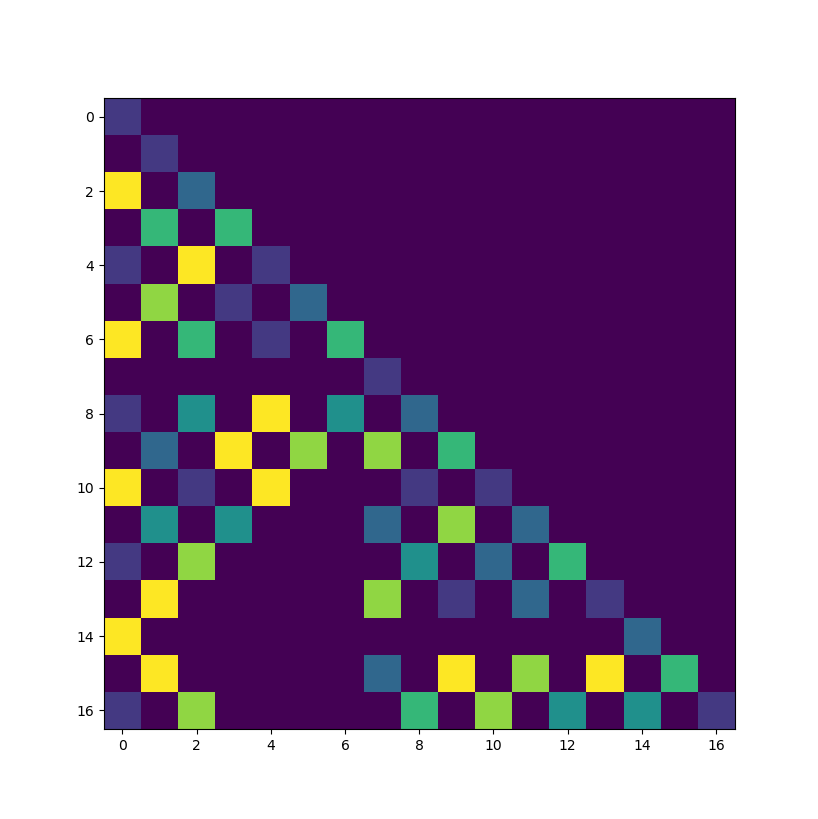
\includegraphics[scale=0.40]{16mod7.png}
  \end{center}

This visual representation corresponds to the table above; every single zero corresponds to a purple square. Already we can see a pattern forming. We extend this analysis to the first $80$ polynomials:

\begin{center}  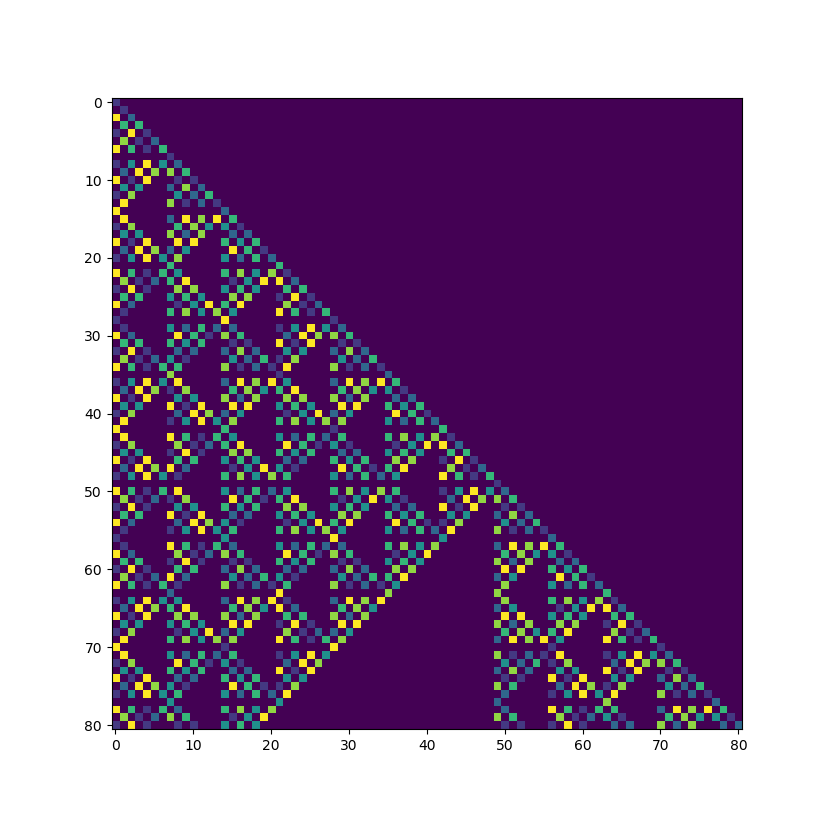
\includegraphics[scale=0.40]{80mod7.png}
\end{center}

All the small triangles are similar to the triangle we saw in the earlier color gradient. Observe furthermore that there is the beginning of an even larger triangle. We extend our analysis once more:

\begin{center}
      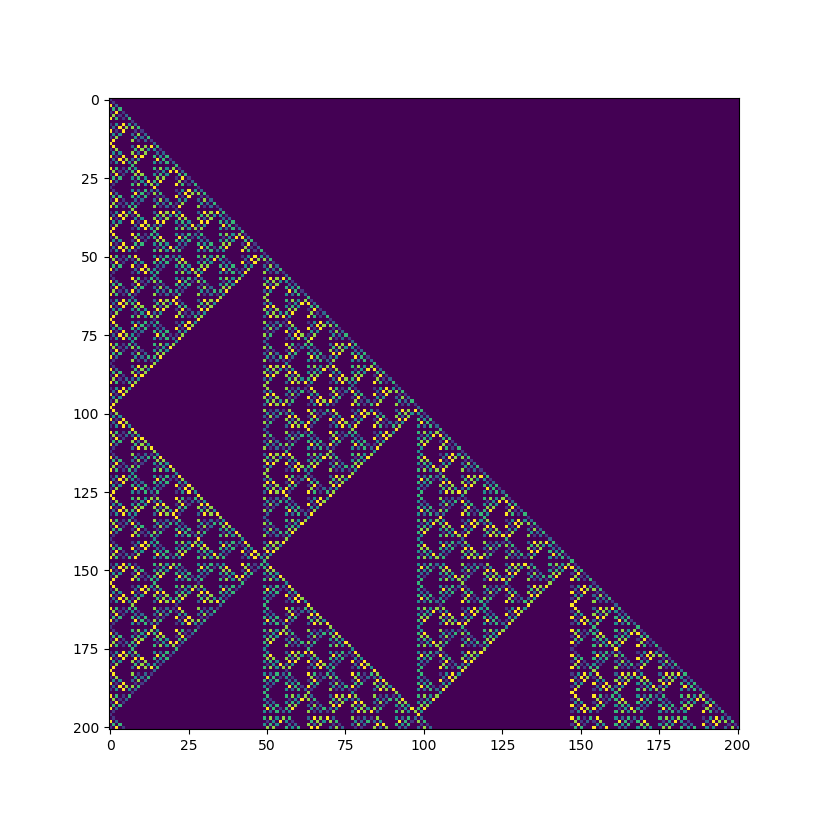
\includegraphics[scale=0.44]{200mod7.png}
\end{center}

We let $J_n$ denote the $n$th triangular number; that is, denote $J_n = \dfrac{n(n+1)}{2}$. We observe that there are $J_6$ small triangles "between" each pair of larger triangles. We conjecture that in general, there are $J_{p-1}$ triangles between pairs of bigger triangles when we consider the coefficients modulo $p$. \newpage

We can see another example of this conjecture when we take a large example for $p = 3$: here are the first $700$ polynomials such that their coefficients are taken $\pmod{3}$:

\begin{center}
      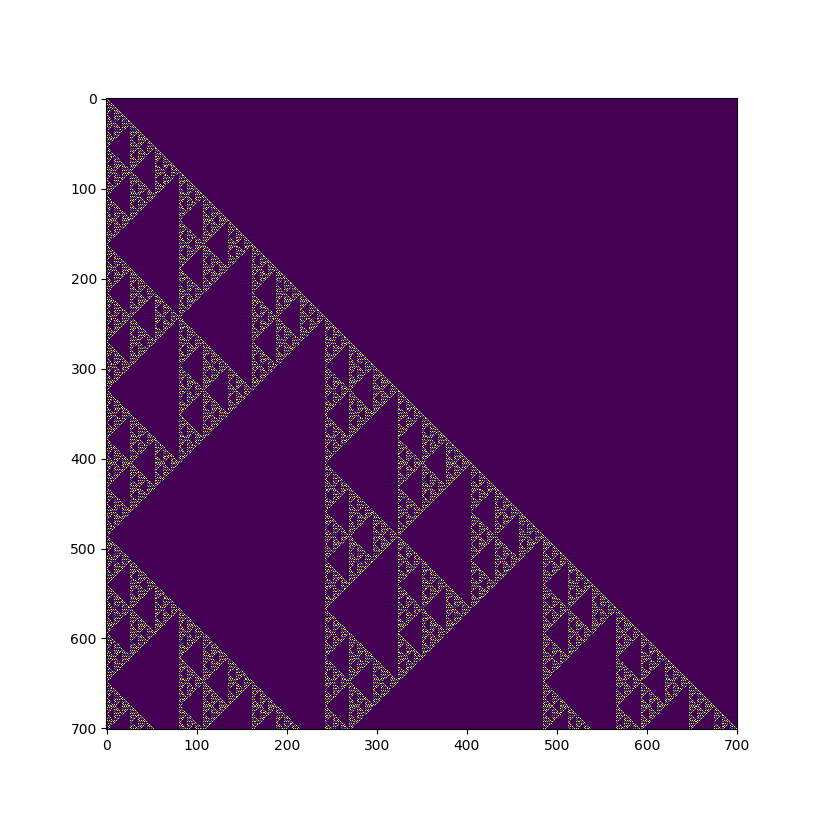
\includegraphics[scale=0.44]{700mod3.png}
\end{center}

Observe that the fractal pattern holds: there are $J_2 = 3$ small triangles "between" every pair of larger triangles. \\

We do not have a proof of this property, but we suspect that it depends on the recurrence we found for $T_n(u)$; the same fractal-like images generate when we repeat this algorithm for $S_n(u)$, which obeys the same recurrence.

\pagebreak
\section{Graphs of $T_n(u)$}
We also want to explore the graphs of the $T_n(u)$, the first 5 of which are as follows:
\vspace{36pt}
 \begin{center}
  \begin{tikzpicture}
   \begin{axis}[
     axis lines = middle,
     xlabel = $u$,
     ylabel = {$T_n(u)$},
     label style={font=\small},
     tick label style={font=\small},
    ]
    \addplot [
     domain=-1:1,
     samples=200,
     color=blue,
    ]
    {x};
   \end{axis}
  \end{tikzpicture} \end{center}
  \begin{center}$T_1(u) = u$ \end{center}

$\linebreak$

 \begin{center}
  \begin{tikzpicture}
   \begin{axis}[
     axis lines = middle,
     xlabel = $u$,
     ylabel = {$T_n(u)$},
     label style={font=\small},
     tick label style={font=\small},
    ]
    \addplot [
     domain=-1:1,
     samples=200,
     color=blue,
    ]
    {2*x^2-1};
   \end{axis}
  \end{tikzpicture}\end{center}
  \begin{center}$T_2(u) = 2u^2 - 1$\end{center}

  $\linebreak$

 \begin{center}
  \begin{tikzpicture}
   \begin{axis}[
     axis lines = middle,
     xlabel = $u$,
     ylabel = {$T_n(u)$},
     label style={font=\small},
     tick label style={font=\small},
    ]
    \addplot [
     domain=-1:1,
     samples=200,
     color=blue,
    ]
    {4*x^3-3*x};
   \end{axis}
  \end{tikzpicture} \[T_3(u) = 4u^3 - 3u\] \end{center}

  $\linebreak$

  \vspace{-18pt}
 \begin{center}
  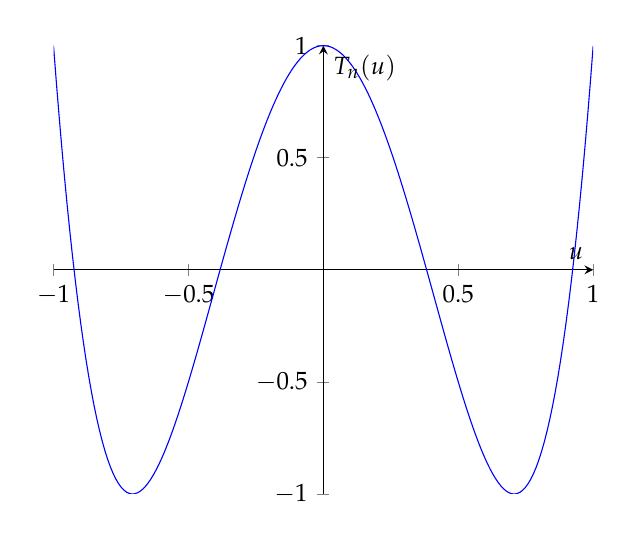
\begin{tikzpicture}
   \begin{axis}[
     axis lines = middle,
     xlabel = $u$,
     ylabel = {$T_n(u)$},
     label style={font=\small},
     tick label style={font=\small},
    ]
    \addplot [
     domain=-1:1,
     samples=200,
     color=blue,
    ]
    {8*x^4-8*x^2+1};
   \end{axis}
  \end{tikzpicture}
  \[T_4(u) = 8u^4 - 8u^2 + 1\]\end{center}

 $\linebreak$

 \vspace{-18pt}
\begin{center}  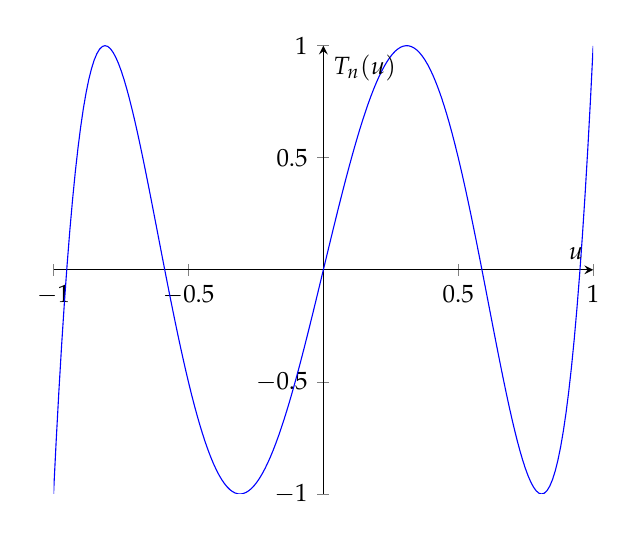
\begin{tikzpicture}
   \begin{axis}[
     axis lines = middle,
     xlabel = $u$,
     ylabel = {$T_n(u)$},
     label style={font=\small},
     tick label style={font=\small},
    ]
    \addplot [
     domain=-1:1,
     samples=200,
     color=blue,
    ]
    {16*x^5-20*x^3+5*x};
   \end{axis}
  \end{tikzpicture}
  \[T_5(u) = 16u^5 - 20u^3 + 5u\]\end{center}

At this point, we overlay the first $8$ graphs for $T_1(u)$ through $T_8(u)$, and observe the following graph:

\begin{center}
  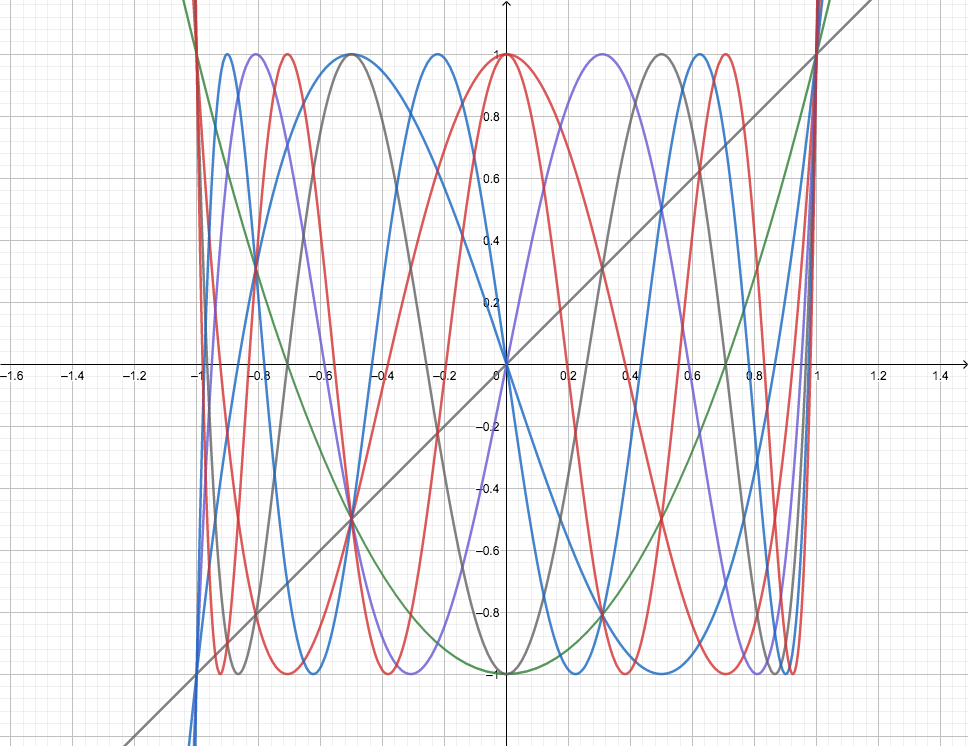
\includegraphics[scale=.44]{pic2.png}
\end{center}

In the above graph, we observe that there are many graphs of polynomials passing through a specific few points. We begin by investigating the concurrences at $\left(-\frac{1}{2},-\frac{1}{2}\right)$ and $\left( -\frac{1}{2}, 1 \right)$.\\

\begin{theorem}
  If $n \in \mathbb{N}$ and $n$ is not a multiple of $3$, then the graph of $T_n(u)$ passes through the point $\left(-\frac{1}{2},-\frac{1}{2}\right)$.
\end{theorem}

\begin{proof}
  As $3$ does not divide $n$, it follows that $n = 3k \pm 1$. Thus $T_n(u) = \cos ((3k\pm 1)x)$. As we want to find $T_n\left( -\frac{1}{2} \right)$, we consider $\cos^{-1} \left(- \frac{1}{2} \right) = \pm \frac{2\pi}{3}$, and as $x = \cos^{-1} u$, we see that $x = \pm \frac{2\pi}{3}$. Plugging this in for $x$ and simplifying yields $-\frac{1}{2}$, as desired.
\end{proof}

\begin{theorem}
  If $n \in \mathbb{N}$ and $n = 3k$ for some $k \in \mathbb{N}$, then the graph of $T_n(u)$ passes through the point $\left( -\frac{1}{2}, 1 \right)$
\end{theorem}

\begin{proof}
  $T_{3n}(-0.5)=\cos\left(3n\cdot \pm \frac{2\pi}{3}\right)=\cos(\pm 2n\cdot \pi)=1$ by the same methods as before.
\end{proof}

We want to look at the number of pairwise intersections between graphs now. Thus we define $I(n,m)$ as the number of intersections of the graphs of $T_n(u)$ and $T_m(u)$, or in other words, the number of solutions to $T_n(u)=T_m(u)$.\\

Two graphs $T_n$ and $T_m$ intersect if $T_n(s) = T_m(s)$. Assume without loss of generality that $n > m$. Let $s = \cos r$, so that $\cos (nr) = \cos (mr)$ and $0 \le r < 2\pi$. Thus $\cos(nr) - \cos(mr) = 0$.\\

Using a trigonometric identity, we see that this is equivalent to
$$2\sin \left( \dfrac{(m+n)r}{2} \right) \sin \left( \dfrac{(n-m)r}{2} \right) = 0.$$

Thus we have two cases: if $\sin \left( \frac{(m+n)r}{2} \right) = 0$, then $\frac{(m+n)r}{2} = k\pi$. This implies, after some algebraic manipulation, that $0 \le k < m+n$. \\

So in total, we have $(m+n)+(n-m)=2n$ solutions. But, we have over-counted some! In particular, we have over-counted $d$ solutions, where $d = \gcd(m+n, m-n)$. This is because such solutions have been counted in both cases.

Since $cos(\theta) = \cos(2\pi - \theta)$, we must exclude the solutions $\theta$ = $0$ and $\pi$ as these are both solutions to $\cos \theta = \cos (2\pi - \theta)$. Hence, we exclude $0$ and $\pi$ if they are solutions, divide the number of solutions by $2$, and add back $0$ and $\pi$ if they are solutions.

If $2|d$, then both $0$ and $\pi$ are solutions. The number of total solutions is then $\frac{2n-d-2}{2}+2 = n-(\frac{d-2}{2})$.

If $2$ does not divide $d$, then $0$ is a solution but $\pi$ is not a solution. Hence, the number of total solutions is $\frac{2n-d-1}{2}+1 = n - (\frac{d-1}{2})$.

Combining these two cases, we see that the number of intersection points $I(n,m)$is $n - \left\lfloor \frac{d-1}{2} \right\rfloor$.

In the other case, we have $\sin \left( \frac{(n-m)r}{2} \right) = 0$. Then in a similar manner we get $0 \le k < n-m$.

\section{Closing Remarks}
There are many topics that we would like to explore in more depth. In the future, we would like to prove the explicit formulas that we conjectured, as well as exploring more explicit formulas and behaviours of this class of polynomials.

\end{document}
